\Chapter{SQL lekérdezések végrehajtása}

\Section{Execution Plan}

A lekérdezés végrehajtási terv elkészítésével információkat nyerhetünk a lekérdezések hatékonyságáról. Ennek segítségével optimalizálhatjuk például egy olyan weboldal működését, mely sok és/vagy bonyolult lekérdezést végez adatbázisból. A hatékonyságot általában indexek hozzáadásával vagy elvételével illetve a táblák kapcsolási sorrendjének módosításával vagy kapcsolási módjának megváltoztatásával segíthetjük elő.

\SubSection{Az \texttt{EXPLAIN} parancs}

\texttt{MySQL} adatbázis kezelő használatakor az Executing Plan -hez szükséges információkat az \texttt{EXPLAIN} parancs segítségével kaphatjuk meg.
Az utasítás megfelelő kifejezéssel együtt használva (\texttt{SELECT}, \texttt{DELETE}, \texttt{INSERT}, \texttt{REPLACE}, \texttt{UPDATE})  információkat jelenít meg az optimalizáló által előállított feldolgozási tervről. Láthatóvá válik például a táblák összekapcsolási sorrendje és a használt index neve.

További információk érhetők el a \texttt{SHOW WARNINGS} használatával.
A \texttt{FORMAT} parancs használható kimeneti formátum választásra. \texttt{TRADITIONAL} az alapértelmezett táblázatos alak illetve \texttt{JSON} ami elnevezésének megfelelő formátumban jelenti meg a kimenetet.

A parancs használata rávilágít arra, hogy hol van szükség indexek használatára a lekérdezés gyorsításához, illetve ellenőrizhetjük, hogy a táblák megfelelő sorrendben vannak -e összekapcsolva. 
\texttt{JOIN} helyett \texttt{STRAIGHT\_JOIN} használatával tippek adhatók az optimalizálónak a táblák kapcsolási sorrendjéről. De a \texttt{STRAIGHT\_JOIN} letiltja a \texttt{semijoin} transzformációkat, így indexelés ebben az esetben nem használható.

\texttt{ANALYZE TABLE} utasítással frissíthetőek a statisztikák, mint a kulcsok számossága. Ez befolyásolhatja az optimalizáló döntéseit. 

% TODO: Ide érdemes kifejteni, MySQL Workbench-es példákkal illusztrálni, hogy hogyan működik a parancs.

\begin{table}[h!]
\centering
\caption{\texttt{EXPLAIN} kimeneti oszlopai}
\medskip
\label{tab:cpuvsgpu}
\begin{tabular}{|p{4cm}|p{4cm}|p{6cm}|}
\hline
oszlop & \texttt{JSON} elnevezés & Jelentése \\
\hline
id & select\_id & A \texttt{SELECT} azonosító \\
\hline
select\_type & - & A \texttt{SELECT} típusa \\
\hline
table & table\_name & a kimeneti sor táblázatának neve  \\
\hline
partitions & partitions & Az egyező partíciók \\
\hline
type & access\_type & \texttt{JOIN} típusa  \\
\hline
possible\_keys & possyble\_keys & választható indexek \\
\hline
key & key & a választott index \\
\hline
key\_len & key\_length & a kiválasztott kulcs hossza \\
\hline
ref & ref & oszlopok az indexhez képest \\
\hline
rows & rows & a vizsgáladnó sorok becslése \\
\hline
filtered & filtered & a szűrt sorok százaléka a tábla állapota szerint \\
\hline
\end{tabular}
\end{table}

\Section{Teszt adatbázis megtervezése}

Az execution plan optimalizálási módnál a kapott információk felhasználásával tudjuk optimalizálni a lekérdezéseket.
Olyan adatbázist kell választanunk ennek kipróbáláshoz amelyben használhatók indexek de nincs feltétlen szükség rájuk, össze kapcsolhatunk több táblát és rendezhetjük az adatokat például növekvő sorrendben. A felhasználási mód miatt kevés dologra kell ügyelnünk a tábláknál, ilyen például a NotNull. A táblák minden eleme INT típusú, és csak a feltöltött adatok értékének intervalluma tér el. Az elsődleges kulcs minden esetben 0 -tól N-1 ig tart.

\begin{figure}[h!]
\centering
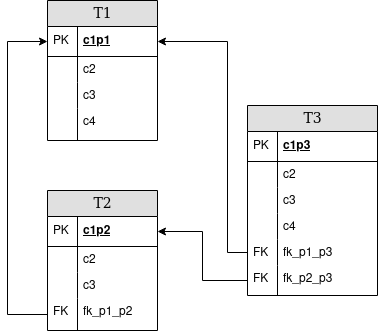
\includegraphics[width=10cm]{images/new_schema.png}
\caption{Adatbázis séma}
\label{fig:schema}
\end{figure}

T1 -es tábla:
\begin{itemize}
\item 100 elemet tartalmaz.
\item c2    random érték [1:2] intervallumon.
\item c3    [1:100]
\item c4    [1:10000]
\end{itemize}
T2 -es tábla:
\begin{itemize}
\item 1000 elemet tartalmaz.
\item c2    [1:100]
\item c3    [1:10000]
\end{itemize}
Létrehozás során ügyeltem arra, hogy minden T1.c1p1 kulcshoz tartozzon legalább egy idegen kulcs ebben a táblában.

T3 -as tábla:
\begin{itemize}   
\item 50.000 elemet tartalmaz
\item c2    [1:100]
\item c3    [1:10000]
\item c4    [1:10]
\end{itemize}
Az idegen kulcsok véletlenszerűen kapcsolódnak a T1 -es és T2 -es táblához.


%Az oszlopnevek számozottak. A \texttt{c3}-\texttt{c5} Az értékeik véletlenszerűen generált egészek, \texttt{c3} $in [0, 100]$, \texttt{c4} $in [0, 10000]$, \texttt{c5} $in [0, 10]$.

T1 kitöltése minta:
\begin{python}
INSERT INTO `thesis`.`T1` (`c1p1`, `c2`, `c3`, `c4`)
VALUES ('0', '1', '50', '150');
\end{python}

\Section{A táblák feltöltése}

Az adatokat egy \texttt{C++} kóddal generáltam \texttt{.csv} formátumba, ügyelve a kapcsolásokra. Majd ezeket a táblákat \texttt{MySQLWorkbench} segítségével importáltam. \texttt{.csv} állományok mintája:
\begin{python}
c1p1, c2, c3, c4
0, 1, 25, 9707
1, 1, 10, 6539
\end{python}
\newpage
\Section{\texttt{EXPLAIN} a gyakorlatban}

A MySQLWorkbench grafikus képeit fogom használni melyeket újraalkottam minőségük miatt. Ez a módszer sokkal jobban szemlélteti miképpen dolgozza fel az utasítást az adatbázis kezelő motorja.

\SubSection{Egyszerű lekérdezés}
Vizsgáljuk a következő lekérdezést:
\begin{python}
SELECT * from thesis.T1 WHERE c3=25; 
\end{python}
\begin{figure}[h!]
\centering
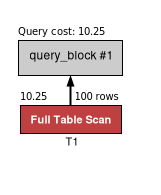
\includegraphics[width=3.5cm]{images/explain/1-1.png}
\caption{Indexelés nélküli lekérdezés}
\label{fig:schema}
\end{figure}

A grafikus Execution Plan az előbbi ábrával állt elő. Láthatjuk, hogy a T1 -es tábla összes sora átvizsgálásra kerül, a c3 megfelelő értékeinek megkereséséhez. Ez egy nagy táblában egy rendkívül költséges művelet lenne. 
Erre nyújt megoldást az indexelés használata.

\begin{python} 
ALTER TABLE  thesis.T1  ADD INDEX (c3);
\end{python}

\begin{figure}[h!]
\centering
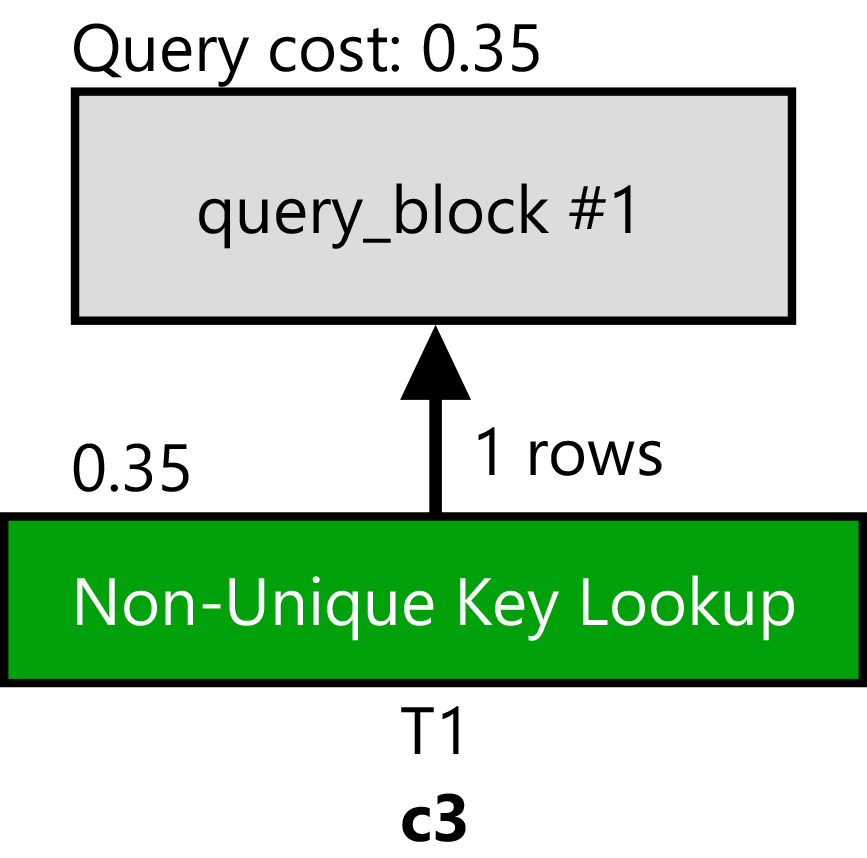
\includegraphics[width=4.2cm]{images/explain/1-2.png}
\caption{Indexelés nélküli lekérdezés}
\label{fig:schema}
\end{figure}

Újra lefuttatva az előző lekérdezést láthatjuk, hogy a költsége a töredékére csökkent, melynek az az oka, hogy nem kell minden cella értékét megvizsgálni.

Parancs az indexek eltávolításához:
\begin{python} 
ALTER TABLE  thesis.T1  DROP INDEX c3;
\end{python}

\newpage
\SubSection{Csoportosítás}

Vizsgáljuk egy kicsit összetettebb lekérdezést: 
\begin{python} 
SELECT MAX(c4), c3, c2 from thesis.T1 WHERE T1.c3=18  group by c2;
\end{python}

\begin{figure}[h!]
\centering
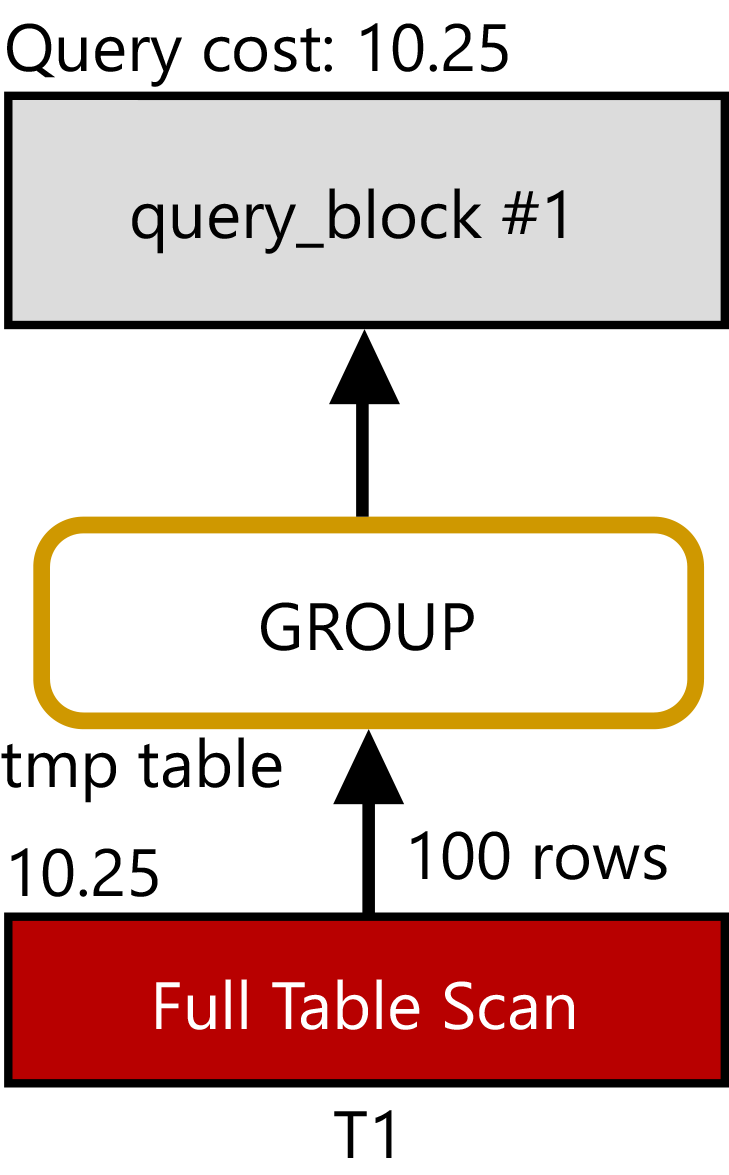
\includegraphics[width=3.5cm]{images/explain/2-1.png}
\caption{Csoportosítás indexelés nélkül}
\label{fig:schema}
\end{figure}

A lekérdezés elemzésénél két problémát fedezhetünk fel. Az egyik a teljes tábla átvizsgálása csak úgy mint az előző esetben. A másik egy ideiglenes tábla létrejötte ami a lekérdezés idejére memóriát foglal.

\begin{figure}[h!]
\centering
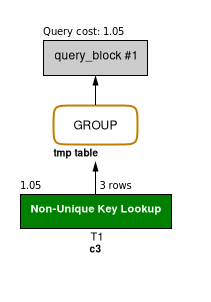
\includegraphics[width=4.2cm]{images/explain/2-4.png}
\hspace{1cm} 
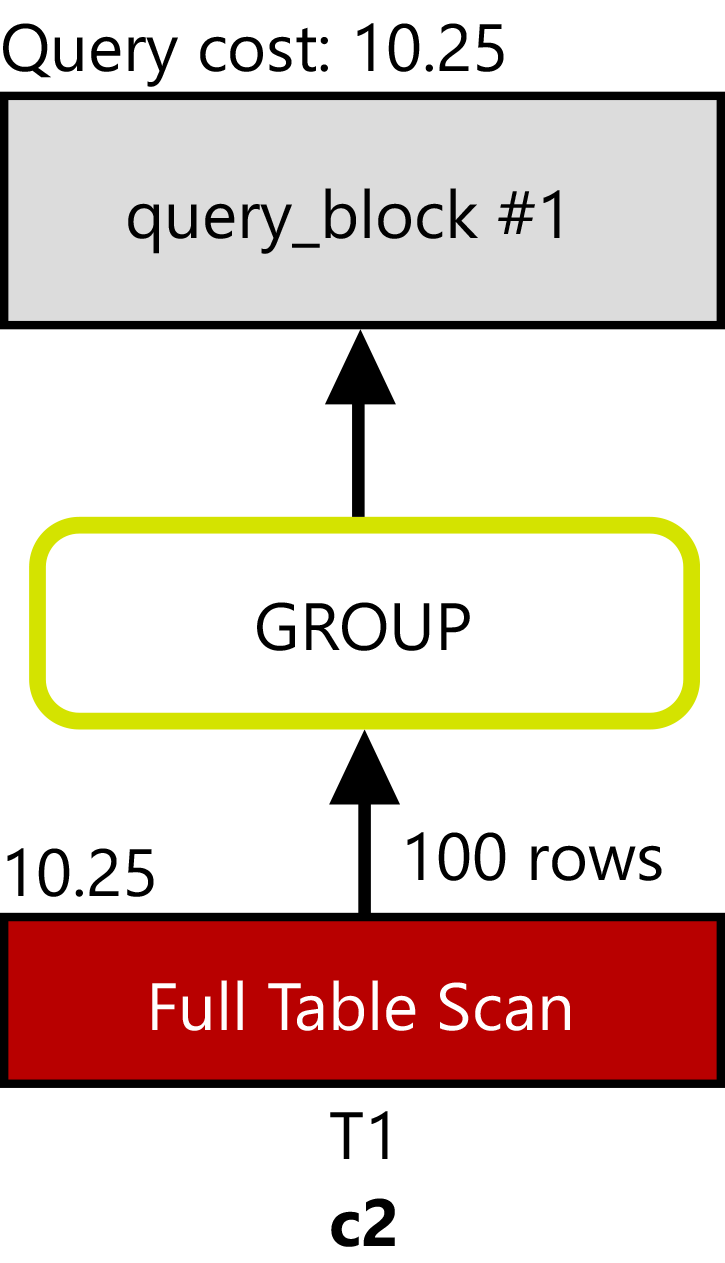
\includegraphics[width=3.51cm]{images/explain/2-2.png}
\hspace{1cm} 
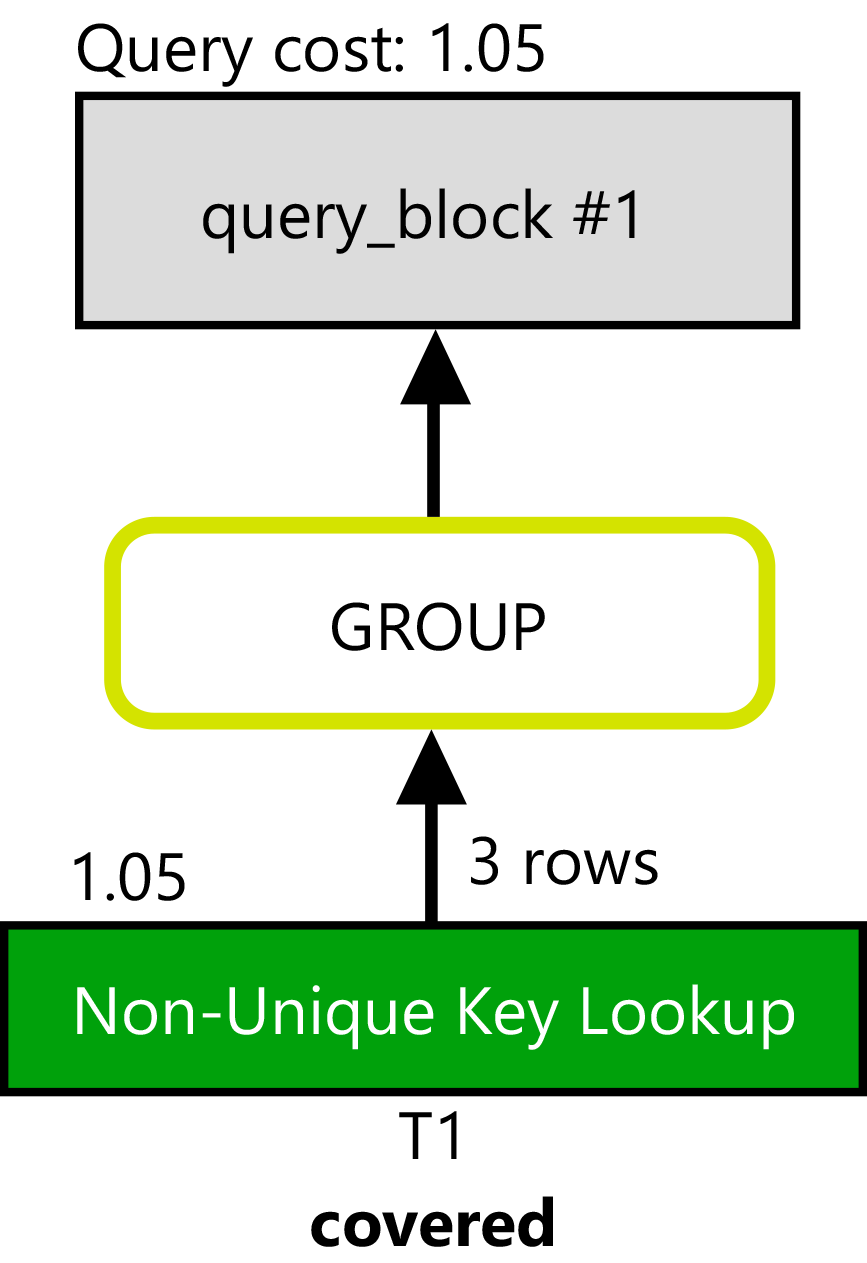
\includegraphics[width=4.2cm]{images/explain/covered.png}
\caption{Indexelések változatai.}
\label{fig:schema}
\end{figure}

Nézzük a következő négy indexelést.
\begin{itemize} 
\item A \texttt{c3} -as oszlop indexelésével az első példához hasonlóan lecsökkent a szűrés költsége.
\item A \texttt{c2} -es oszlop indexelésével az ideiglenes tábla nem jön létre lekérdezés közben.
\item \texttt{c2} és \texttt{c3} külön indexelése esetén ugyan az történik mint \texttt{c3} indexelésekor.
\item \texttt{c2} és \texttt{c3} közös indexelésével egyesíthetjük és két előnyt és így a lekérdezés optimális sebességű és memória igényű lesz.
\end{itemize} 
Kevert index létrehozása és törlése:
\begin{python}
ALTER TABLE T1 ADD INDEX covered (c3,c2);
ALTER TABLE thesis.T1 DROP INDEX covered;
\end{python}

\SubSection{Kapcsolt táblák}

Ez a lekérdezés már összetettebb, annak érdekében, hogy látszódjon a lekérdezés optimalizáló mely esetekben milyen sorrendben kapcsolja össze a táblákat.
\begin{python}
SELECT T1.c3, T2.c2, T3.c3 FROM T3 JOIN T2 JOIN T1 
	ON (T1.c1p1 = T2.fk_p1_p2 AND T2.c1p2 = T3.fk_p2_p3) 
	WHERE  T3.c4=5 AND T1.c2 = 1 ;
\end{python}

\begin{figure}[h!]
\centering
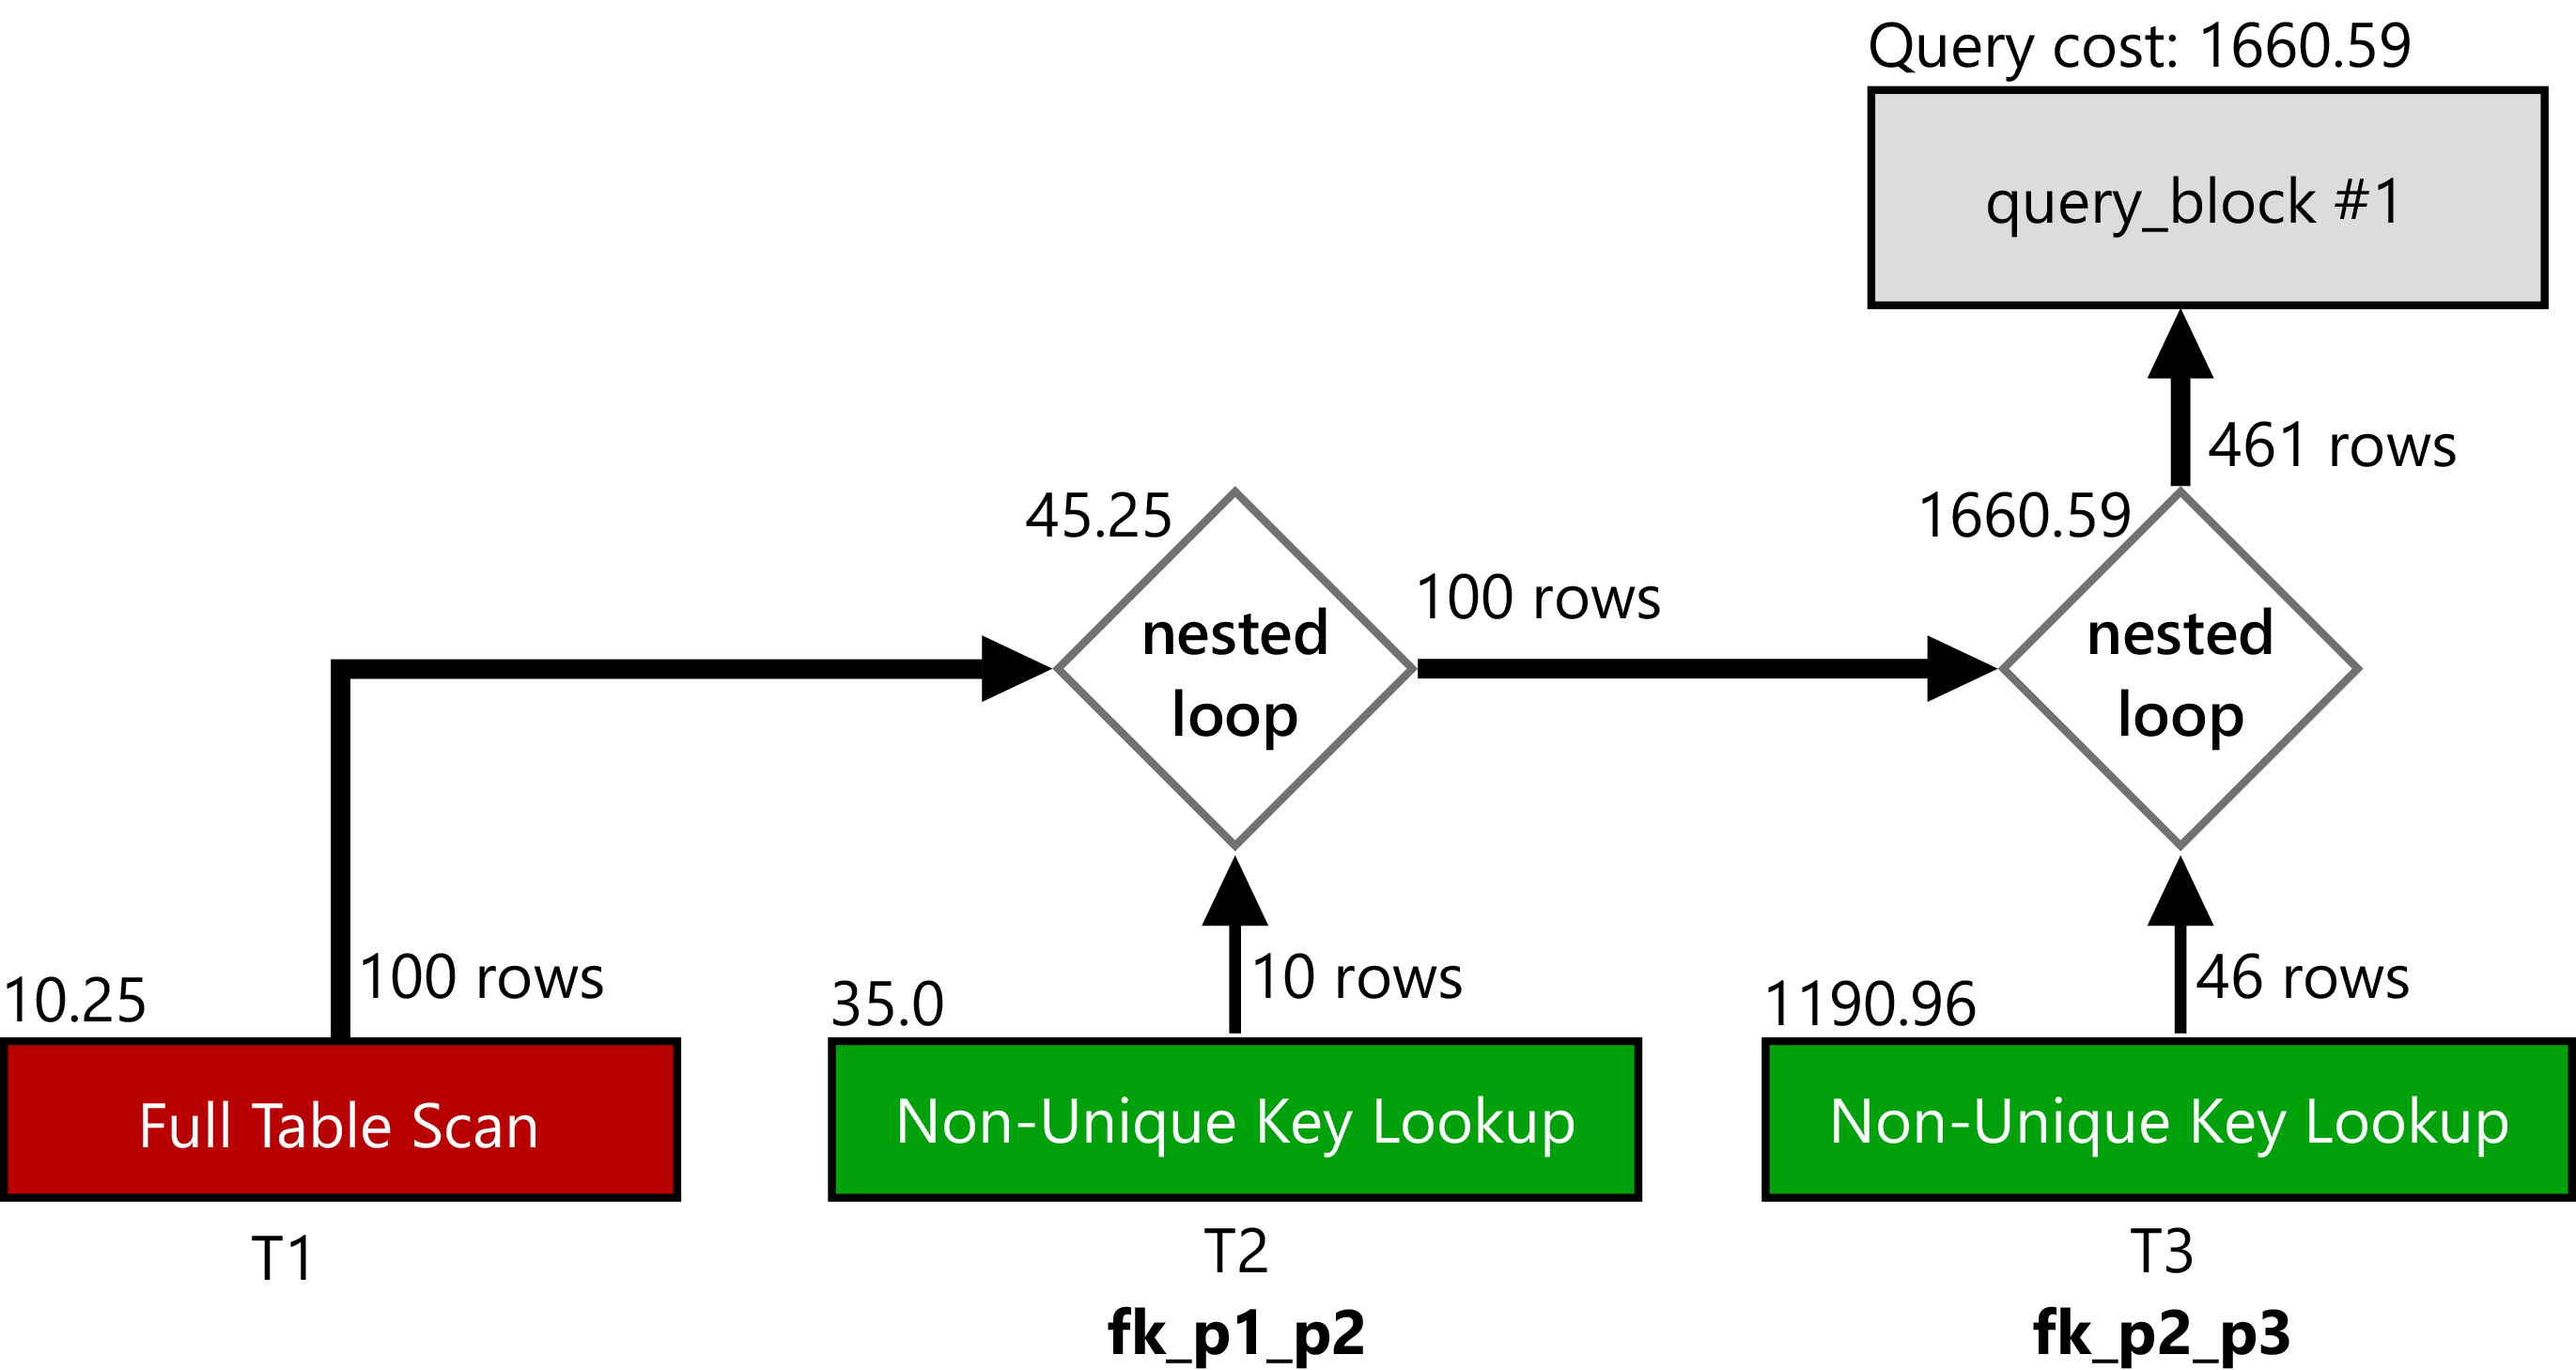
\includegraphics[width=14cm]{images/explain/3-1.png}
\caption{JOIN indexelés nélkül}
\label{fig:schema}
\end{figure}

Látható, hogy a kapcsolások sorrendje nem egyezik a lekérdezésben megadott sorrenddel, illetve látjuk az előbbi példákból már jól ismert teljes tábla átvizsgálás hibáját.
Miután \texttt{T3} -as tábla vizsgált oszlopát indexeléssel láttam el, szinte ugyan ezt az eredményt kaptam, leszámítva két értéket. \texttt{T3} -nál a költség 1190.96 -ról 1198.86 -ra nőtt illetve a 2. \texttt{nested loop} -nál a sorok száma 450 re csökkent.

\newpage
A következő vizsgálatban csak \texttt{T1} \texttt{c2} -es oszlopa indexelt.

\begin{figure}[h!]
\centering
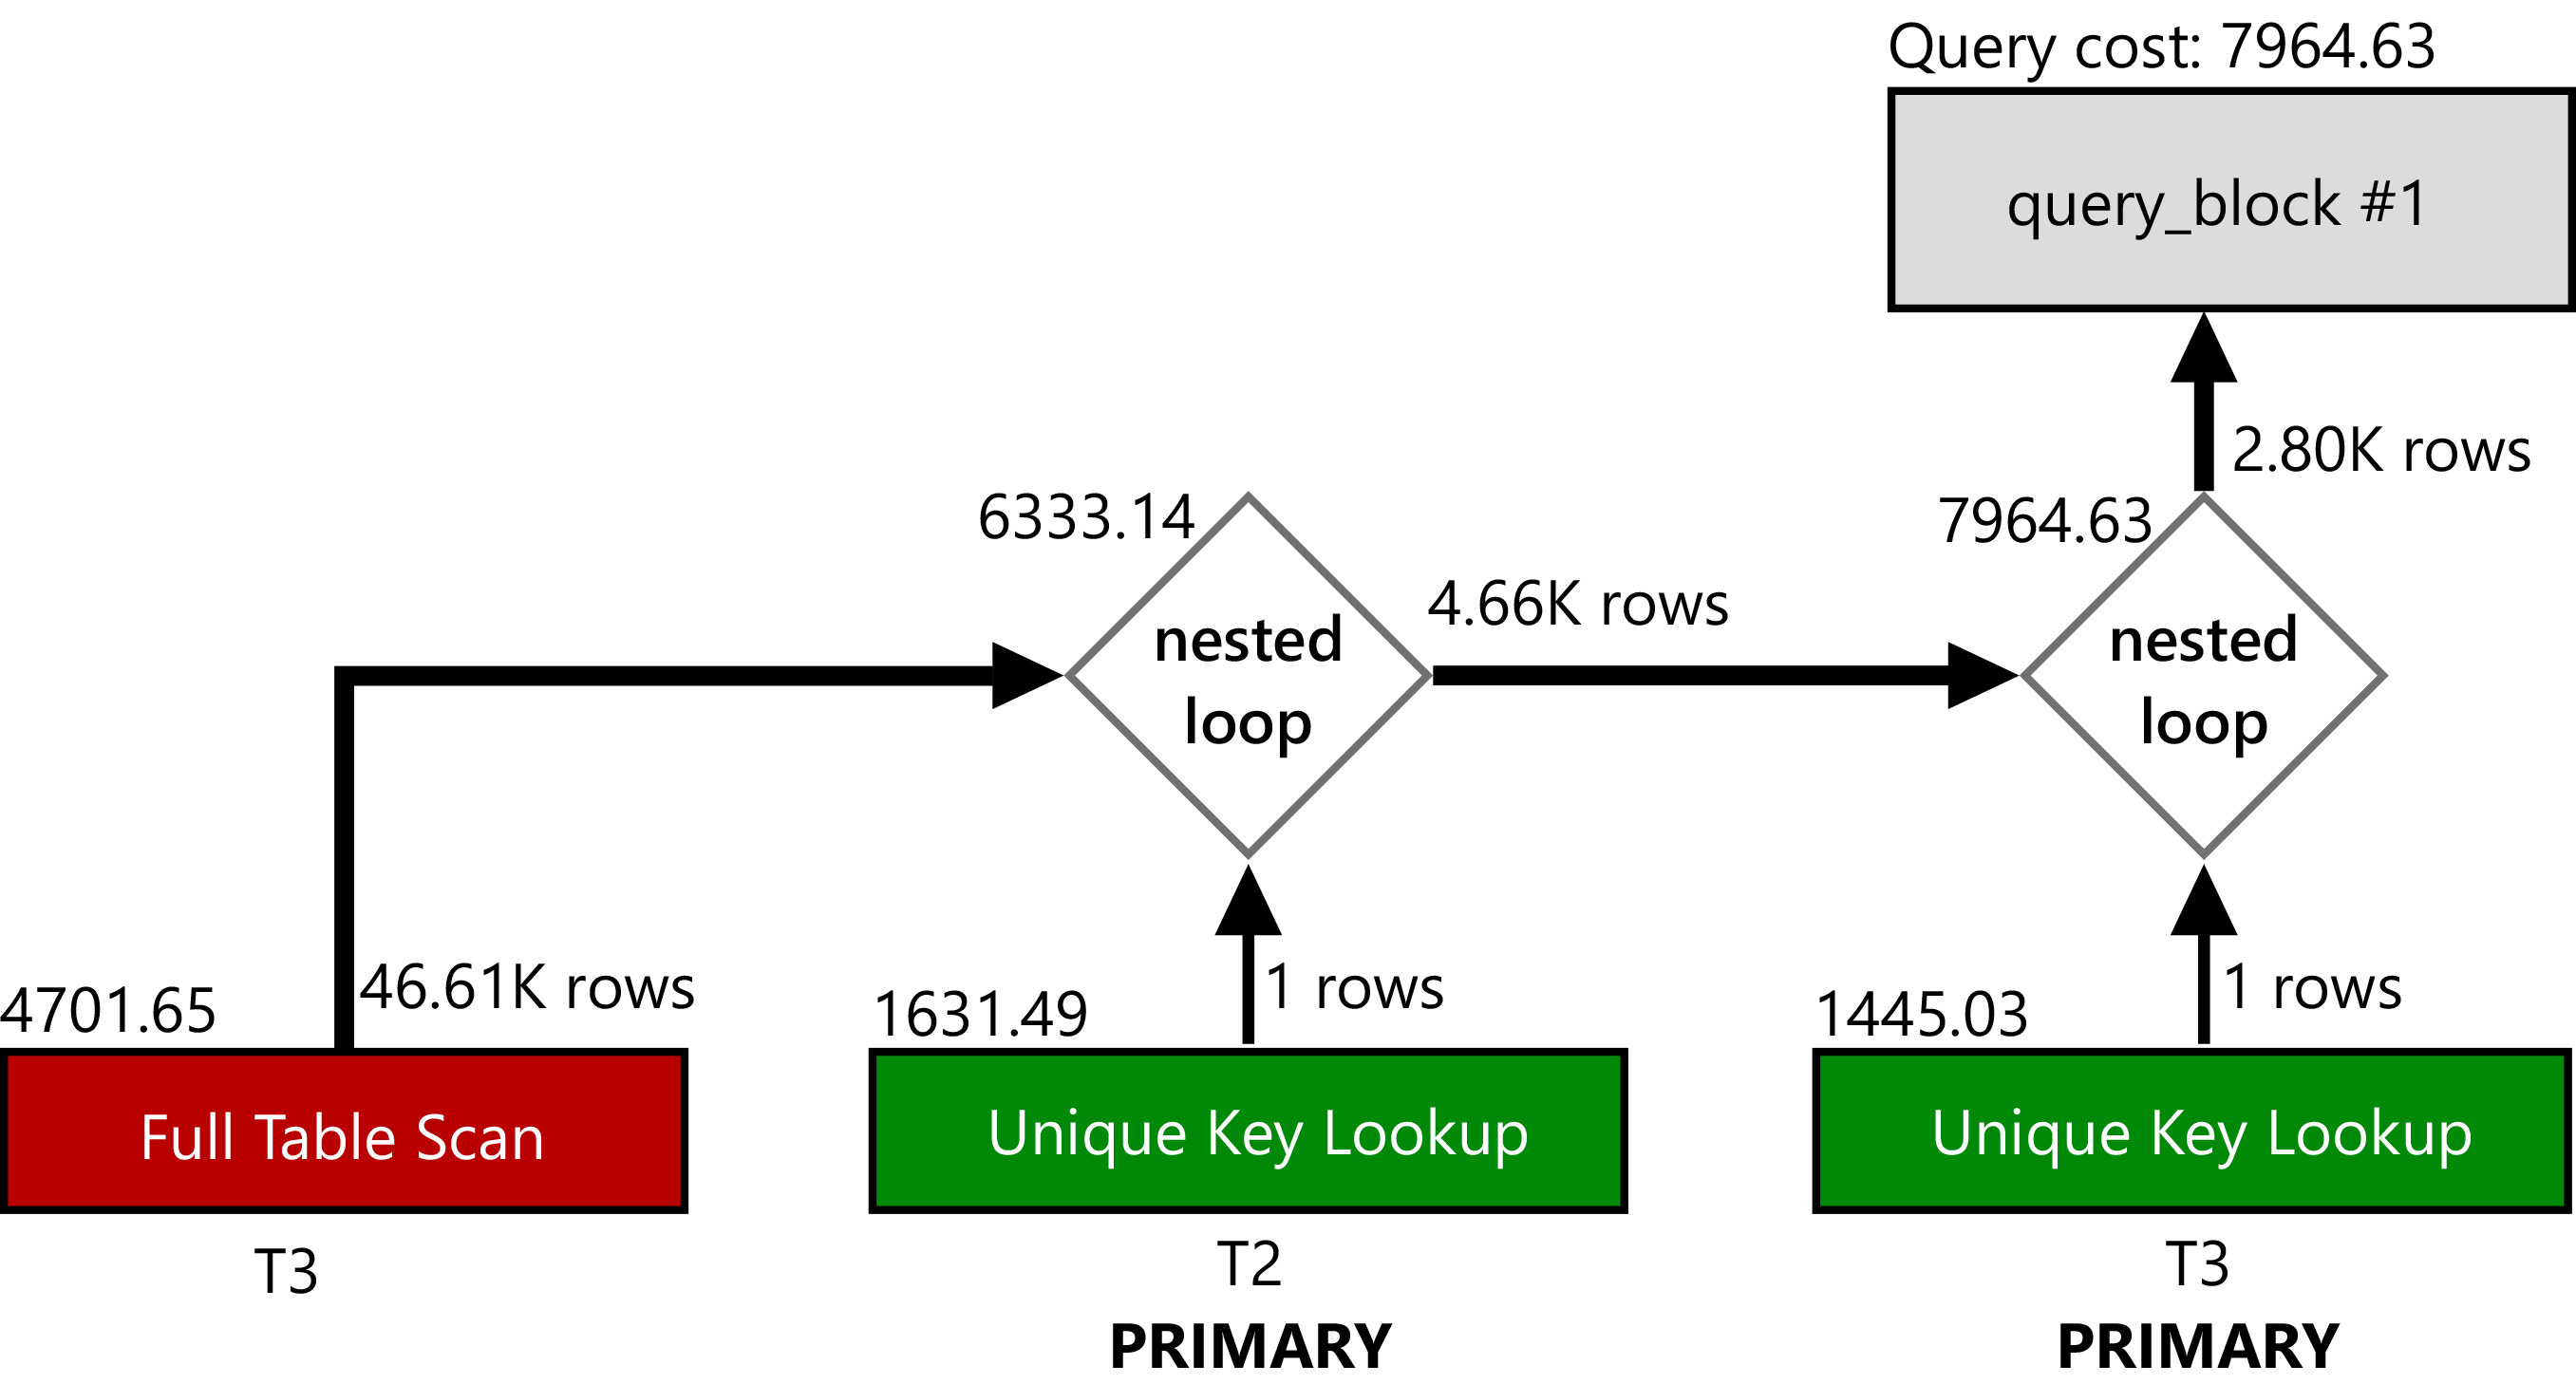
\includegraphics[width=14cm]{images/explain/3-2.png}
\caption{JOIN T1.c2 és T3.c4 indexelésével}
\label{fig:schema}
\end{figure}

Az eredményből az látszik, hogy megváltozott a táblák kapcsolási sorrendje. A query első lépésben szűri a \texttt{T3} -as táblát és csak utána kapcsolja hozzá a többit. A másik dolog amit meg lehet figyelni, hogy nem az idegen kulcs szerepel a használt indexnél, hanem az elsődleges. De ez is a sorrend változás következménye.

A negyedik vizsgálatban mind a két tábla használt oszlopát indexekkel láttam el.
\begin{figure}[h!]
\centering
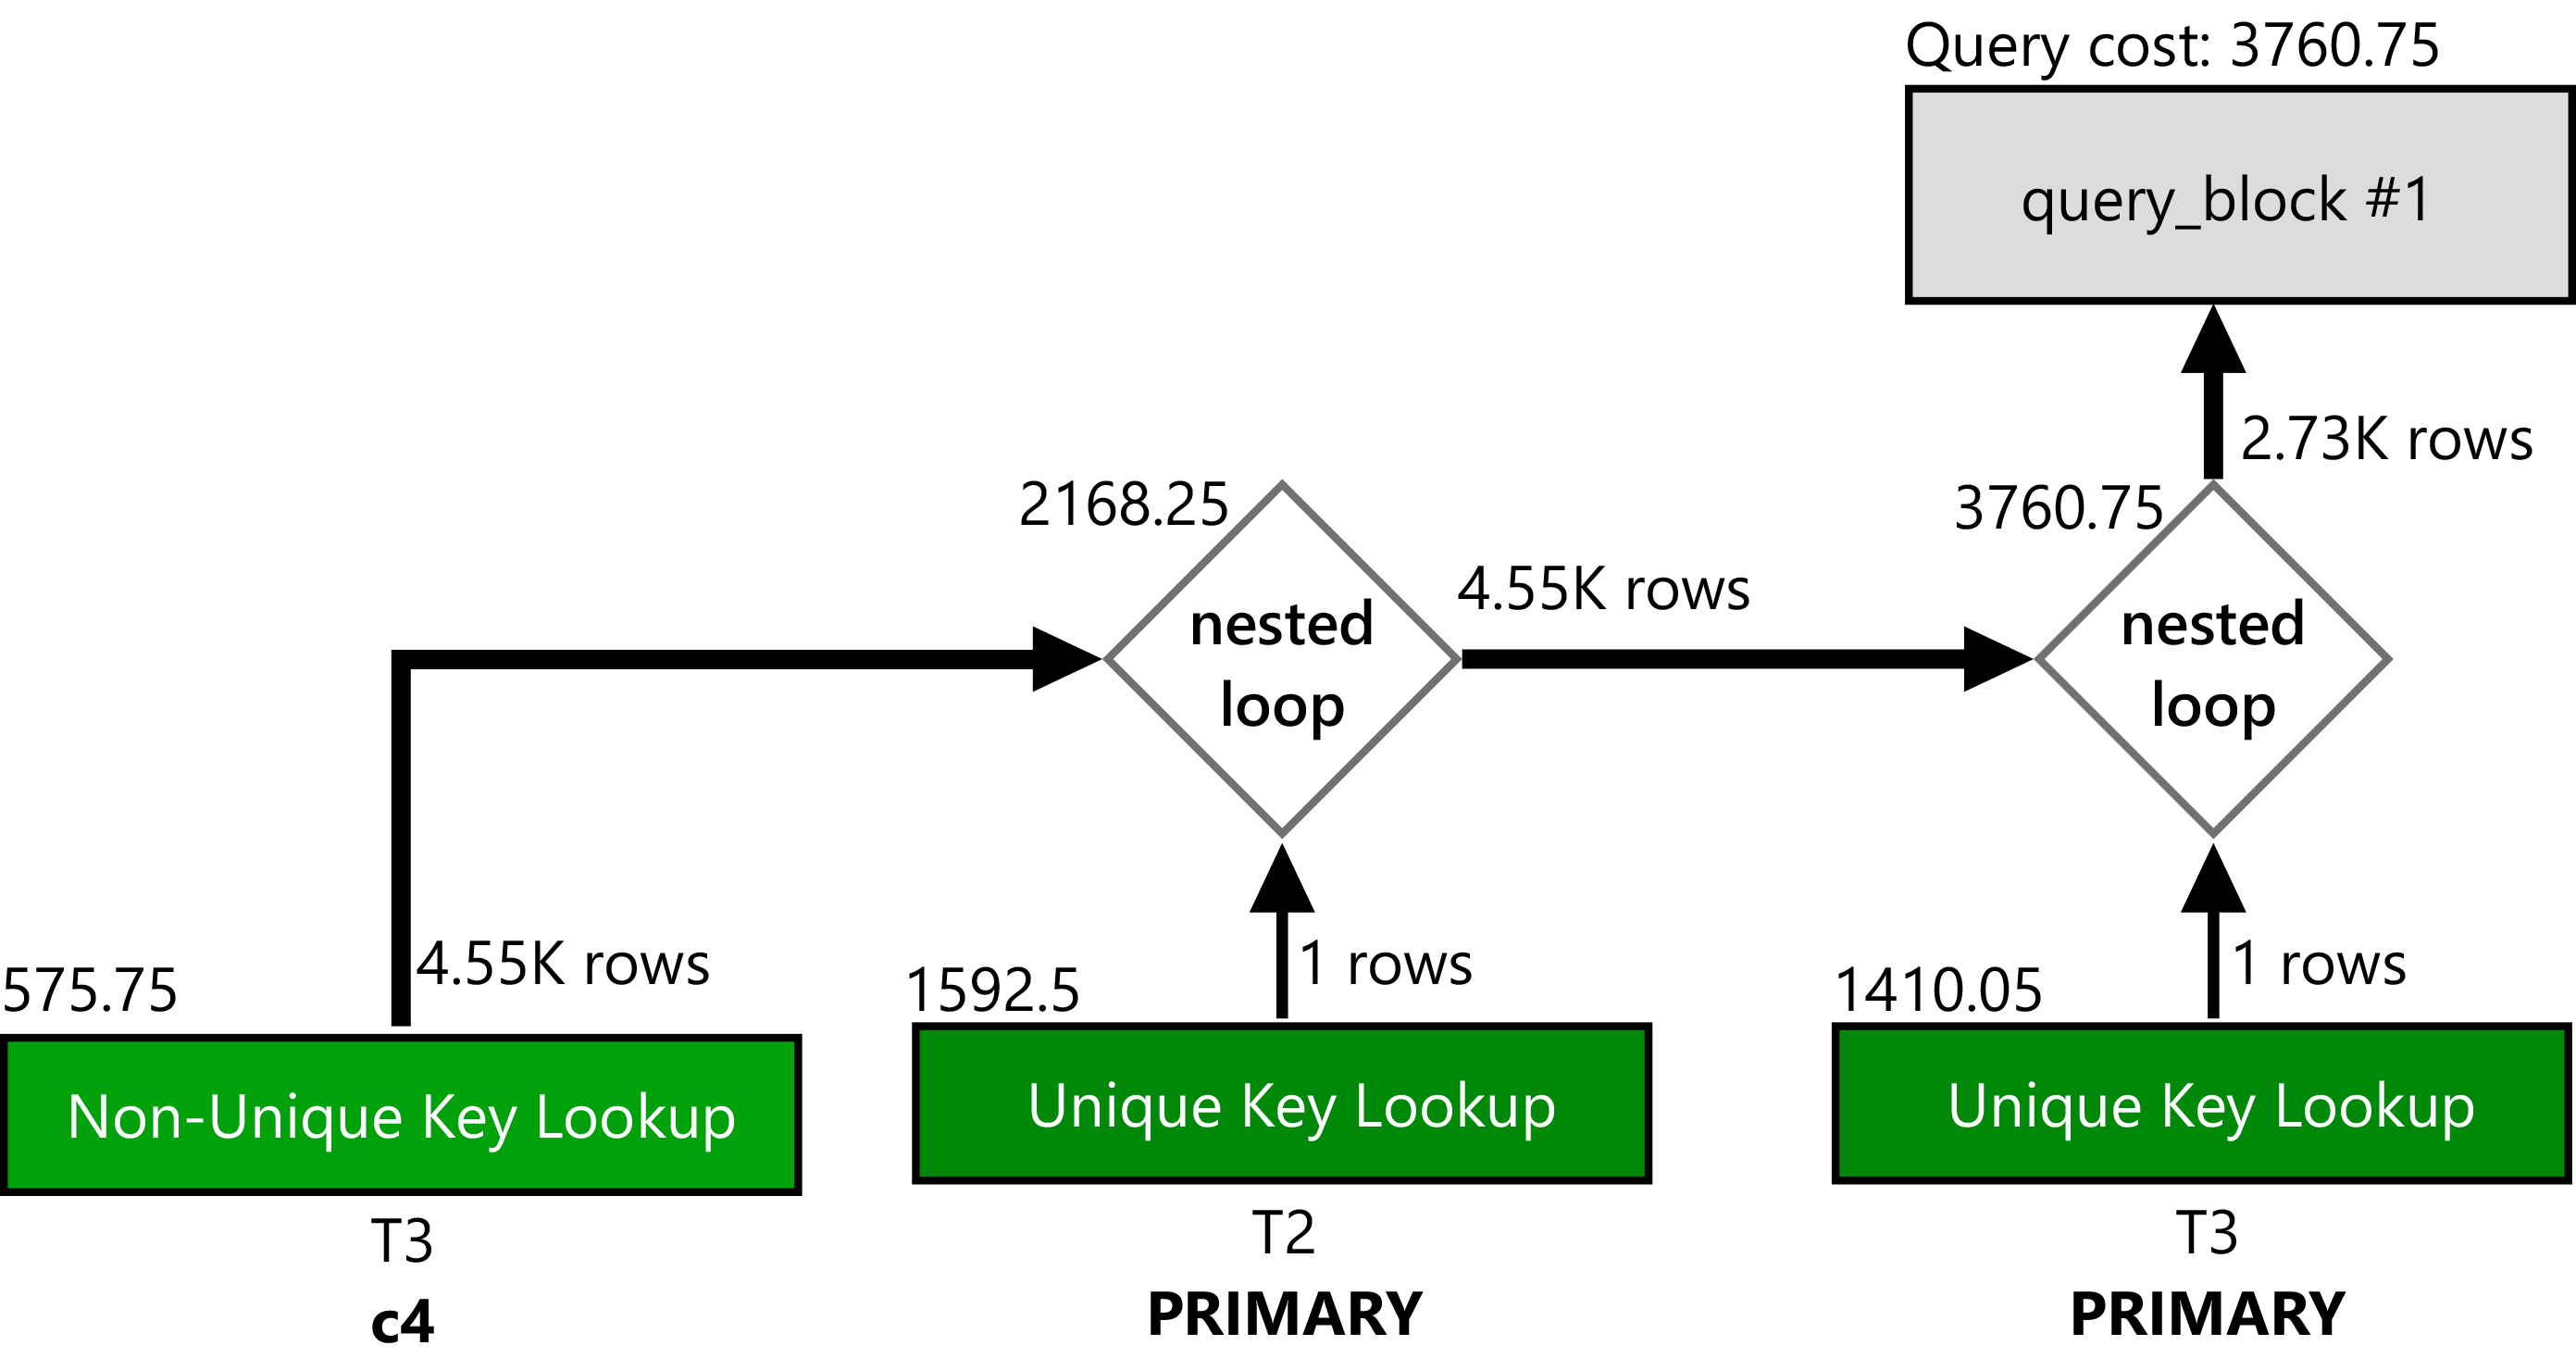
\includegraphics[width=14cm]{images/explain/3-3.png}
\caption{JOIN T1.c2 indexelésével}
\label{fig:schema}
\end{figure}

Ezen az ábrán egy azt a változást láthatjuk az előzőhöz képest, hogy a \texttt{T3} as táblánál, az optimalizáló mind a két indexet használja, ugyanis a sorrend változatlan maradt, és \texttt{T3} alatt megjelent a használt index neve.
Az ábrákon látható query cost megtévesztő lehet, hisz arra enged következtetni, hogy nem érdemes indexelést használni ebben az esetben, viszont a lekérdezés sebességének vizsgálata egyértelműen mutatja, hogy az indexek használata jelentős sebesség növekedéssel járt. 
